\documentclass[12pt,letterpaper, onecolumn]{exam}
\usepackage{amsmath}
\usepackage{amssymb}
\usepackage{graphicx}
\usepackage{caption}
\usepackage{tikz}
\graphicspath{ {.} }
\usepackage[lmargin=71pt, tmargin=1.2in]{geometry}
\lhead{Mustafa Rashid\\}
\rhead{Problem Set 3\\}
\chead{\hline} 
\thispagestyle{empty} 
\newcommand*{\setdef}[1]{\left\{#1 \right\}} 
\usepackage[left=2.00cm, right=1.00cm]{geometry}


\begin{document}
	
	\begingroup  
	\centering
	\LARGE Multi-variable Calculus\\
	\LARGE Problem Set 3\\[0.5em]
	\large \today\\[0.5em]
	\large Mustafa Rashid\par
	\large Fall 2024\par
	\endgroup
	\rule{\textwidth}{0.4pt}
	\pointsdroppedatright
	\printanswers
	\renewcommand{\solutiontitle}{\noindent\textbf{Ans:}\enspace}  
	
	

	\begin{questions}
		
		\question Is the following statement true or false? If true, briefly justify it; if false, proveide a specific counter-example
		\begin{quote}
			\textit{In a table of values for a linear function, the columns have the same slope as the rows.}
		\end{quote}	
		
		\begin{solution}
			False. Consider the following table of values for the linear function $z=-0.5-x+2y$\\
			The column with $y$ fixed at 2 has a slope of $-1$ while the row with $x$ fixed at 2 has a slope of 2.\\
			\begin{tabular}{ c c c}
				$x$/$y$ & 1.5 & 2.0\\
				2 & 0.5 & 1.5\\
				3 & -0.5 & 0.5\\
			\end{tabular}

		\end{solution}
		
		\question The pressure of gas in  a storage container, in atmosphere, is given by
		$$P=f(n,T,V)=\frac{82nT}{V},$$
		where $n$ is the amount of gas, in kilomoles, $T$ is the temperature of the gas, in Kelivn, and $V$ is the volume of the storage container, in liters.
		\begin{parts}
			\part Find a formula for the \textbf{level surface} of $f$ containing the points $(n,T,V)=(1,270,20)$, and explain the significance of this surface in terms of pressure.
			\part Find another point on the level surface in part (a), and explain the significance of this point in terms of pressure.
		\end{parts}
		\pagebreak
		\begin{solution}
			\begin{parts}
				\part  $$f(1,270,20)=\frac{82\cdot1\cdot270}{20}=1107$$
				$$P=1107 \textrm{ atmospheres}$$
				$$\frac{82nT}{V}=1107$$
				$$f(n,T,V)=1107$$
	
				The level surface corresponds to all points where the pressure is equal to 1107 atmospheres.
				\part Let V=8 litres and T=18 Kelvin, then from the formula of the level surface we have $f(n,18,8)=1107$
				$$\frac{82\cdot n\cdot18}{8}=1107$$
				$$n=\frac{1107\cdot8}{18\cdot82}$$
				$$n=6 \textrm{ kilomoles}$$
				Since this is a point on the level surface $f(n,T,V)$ the resulting pressure must be equal to 1107 atmospheres
			\end{parts}
		\end{solution}
		
		\question Resolve the following vectors into components. In other words, write down the vector explicitly (either in angle bracket notation or with $\vec{i},\vec{j},\vec{k}$). NOTE: $\mathbb{R}^{2}$ refers to 2D-space while $\mathbb{R}^{3}$ refers to 3D-space.
		\begin{parts}
			\part The vector in $\mathbb{R}^{2}$  of length 2 pointing up and to the right at an angle of $\frac{\pi}{4}$ with respect to the positive $x$-axis
			\part The vector in  $\mathbb{R}^{3}$ of length 1 lying in the $xz$-plane pointing upward at an angle $\frac{\pi}{6}$ with respect to the positive $x$-axis, 
			\end{parts}. 
		
		\begin{solution}
			\begin{parts}
				\part We are looking for a vector $<a,b>$ where $\sqrt{a^2+b^2}=2$ and  $a>0, b>0$\\
				\begin{tikzpicture}
					\coordinate (a) at (0,0);
					\coordinate (b) at (4,0);
					\coordinate (c) at (4,2);
					\draw (a) -- (b)node[midway, below]{a} -- (c)node[midway,right]{b} -- (a)node[midway,left, above]{2}; % Triangle.
				
					\draw (a) node[anchor=east,align=center] {$\theta=\frac{\pi}{4}$};
					\draw (b) node[anchor=west,align=center] {};
					\draw (c) node[anchor=south]{};
				\end{tikzpicture}\\
				We know from the fact that the vector makes an angle of $\frac{\pi}{4}$ with the positive $x$-axis and trigonometry that the following is true
				$$cos\theta=\frac{a}{2}$$
				$$a=2cos\theta=2cos(\frac{\pi}{4})$$
				$$=\sqrt[]{2}$$
				$$sin\theta=\frac{b}{2}$$
				$$b=2sin\theta=2sin(\frac{\pi}{4})$$
				$$=\sqrt[]{2}$$
				
				The vector is $<\sqrt{2},\sqrt[]{2}>$
				\part Because the vector lies in the $xz$-plane then $y=0$\\
				\begin{tikzpicture}
					\coordinate (a) at (0,0);
					\coordinate (b) at (4,0);
					\coordinate (c) at (4,2);
					\draw (a) -- (b)node[midway, below]{$x$} -- (c)node[midway,right]{$z$} -- (a)node[midway,left, above]{1}; % Triangle.
					
					\draw (a) node[anchor=east,align=center] {$\theta=\frac{\pi}{6}$};
					\draw (b) node[anchor=west,align=center] {};
					\draw (c) node[anchor=south]{};
				\end{tikzpicture}\\
				We know from the fact that the vector makes an angle of $\frac{\pi}{6}$ with the positive $x$-axis and trigonometry that the following is true
				$$cos\theta=\frac{x}{1}}$$
				$$x=cos(\frac{\pi}{6})$$
				$$=\frac{\sqrt{3}}{2}$$
				$$sin\theta=\frac{z}{1}$$
				$$z=sin(\frac{\pi}{6})$$
				$$=\frac{1}{2}$$
				
				The vector is $<\frac{\sqrt[]{3}}{2}},0,\frac{1}{2}>$
			\end{parts}
		\end{solution}
		
		\question Figure 1 shows the graph of the function $f(x,y)$ on the domain $0\leq x\leq4$ and $0\leq y \leq4$. Use the graph to rank the following quantities in order from \textbf{smallest to largest}
		$$f_x(3,2),f_x(1,2),f_y(3,2),f_y(1,2),0$$
		Explain your reasoning.\\
		\makebox[0pt][l]{
			\begin{minipage}{\textwidth}
				\centering
				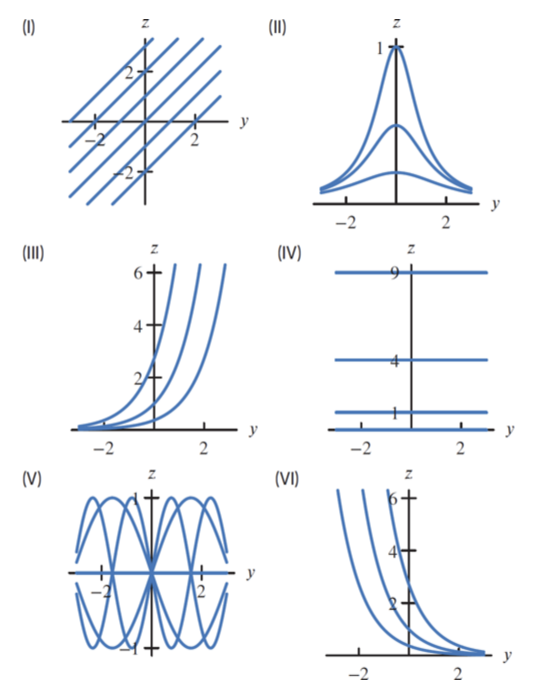
\includegraphics[width=.4\textwidth]{question4}
				\captionof{figure}{}
				\label{fig:fig1}
			\end{minipage}
		}
		

		\begin{solution}
		 At the point $(1,2)$ the partial derivative with respect to $x$ is negative but it is more negative than the partial derivative with respect to $x$ at the point $3,2$ as the graph is dips faster around $(1,2)$ than $(3,2)$ in the $x$-direction. At the point $(1,2)$ the partial derivative with respecrt to $y$ is positive as the graph rises upwards. The same is true for the point $(3,2)$ but the graph rises upwards much less rapidly than at $(1,2)$. The smallest value is where the rate of change is most negative while the largest value is where the rate of change is most positive. Therefore, the order from smallest to largest will the following:
		 $$f_x(1,2),f_x(3,2),0,f_y(3,2),f_y(1,2)$$
		\end{solution}
	\end{questions}
\end{document}
